\chapter{Идентификация системы связанных релаксационных генераторов}

\newcommand{\RelaxBjtIi}{системы из трёх связанных релаксационных генераторов на паре комплиментарных транзисторов}
\newcommand{\RelaxShIi}{системы из трёх связанных релаксационных генераторов на основе триггеров Шмидта}

\section{Реласкационные генераторы: применение, модели}

Применение: собственно генераторы, источники питания.

Элементная база, задачи. Почему возможны хаотические режимы

Не совсем прототип: Kennedy


\cite{mishenko_du_small_relax}

\section{Система из трёх связанных релаксационных генераторов на паре комплиментарных транзисторов}
\label{atu:sec:relax3d}

Основы

\begin{figure}[htb!]
  \centerline{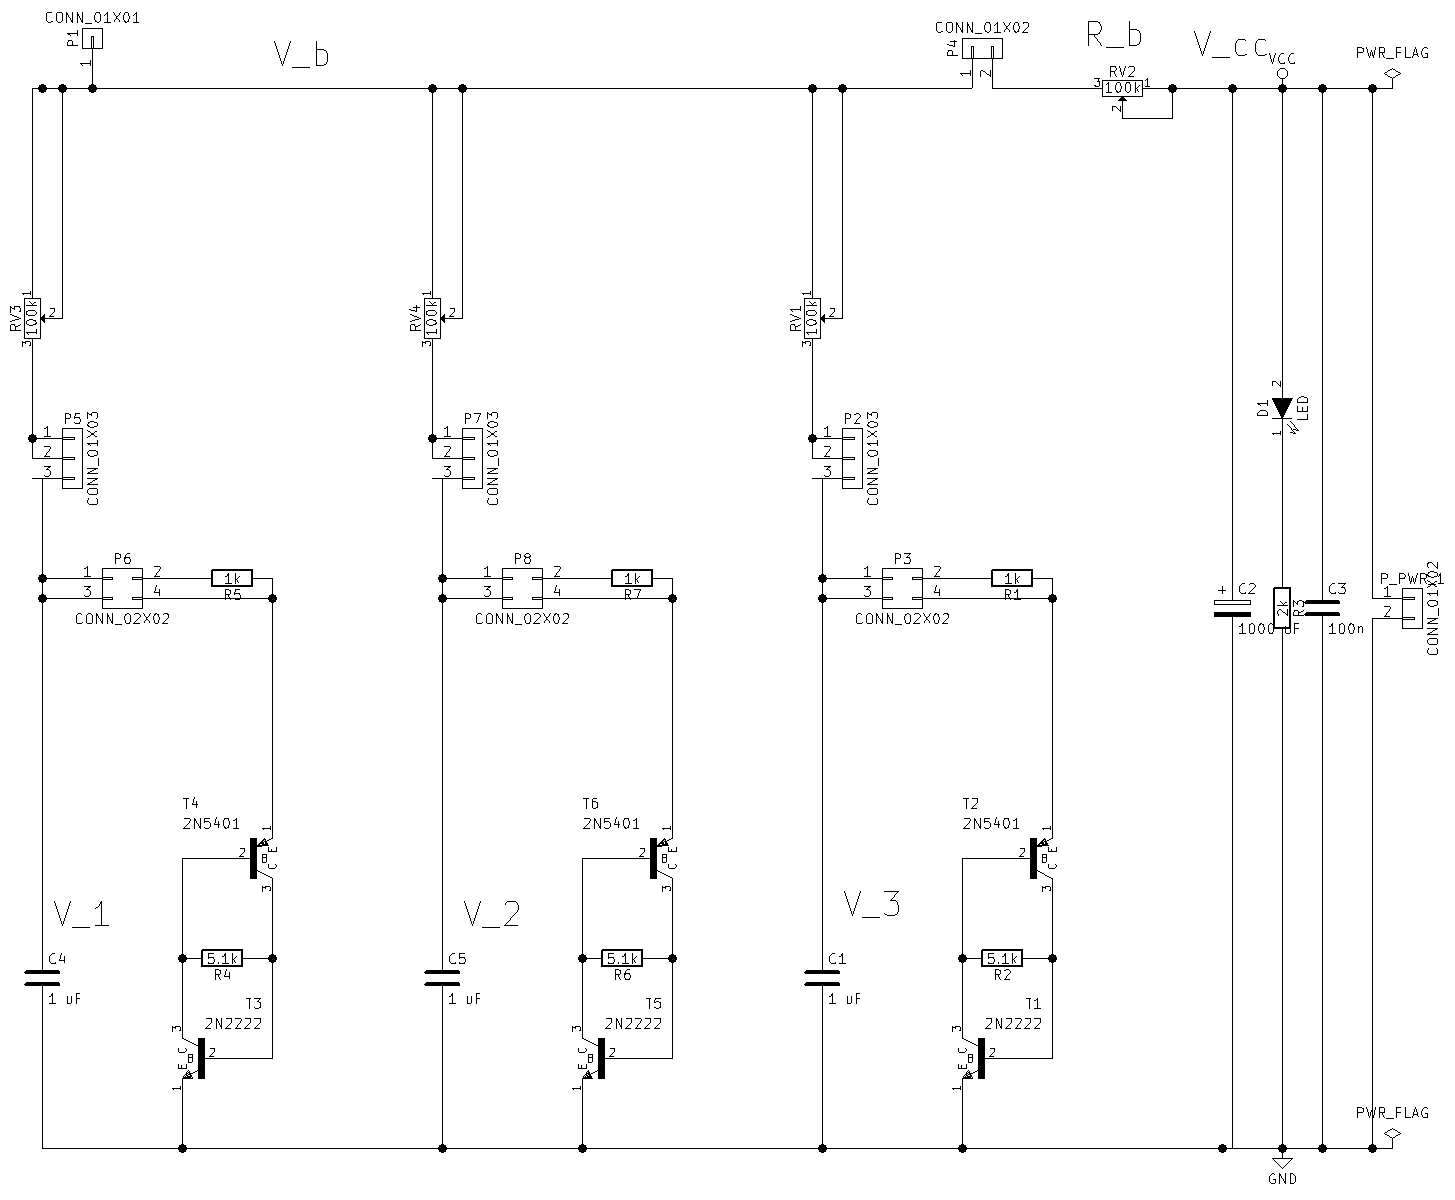
\includegraphics[width=0.7\textwidth]{p/relax3d_2bjt_schem.png} }
  \caption{Электрическая схема \RelaxBjtIi}
  \label{atu:f:relax3d_schem}
\end{figure}

Динамика.

\section{Система из трёх связанных релаксационных генераторов на основе триггеров Шмидта}
\label{atu:sec:relax3ds}

Схемотехническая реализация системы связанных релаксационных генераторов,
рассмотренная в разделе \ref{atu:sec:relax3d}, несмотря на ряд достоинств,
обладает определёнными недостатками. В первую очередь, следует отметить
тот факт, что при относительно высоких значениях величины $R_b$,
как раз при которых связь между отдельными генераторами становится существенной,
релаксационный элемент переключается из колебательного режима в режим
стабилизации напряжения, что не соответствует предназначению данной схемы.
Более того, в этих условиях зависимость тока от напряжения близка к экспоненциальной,
что затрудняет создание адекватной модели. При этом малые изменения параметров,
например, вызванные температурной нестабильностью, приводят к значительным изменением
тока, что также негативно сказывается на адекватности. Ещё один недостаток
заключается в том, что существующими элементами можно изменять напряжение срабатывания
в достаточно узком диапазоне, что затрудняет проведение как экспериментов,
так и моделирования в широком диапазоне параметров. В свою очередь,
это ставит вопросы о границах применимости модели, на которые сложно
ответить, опираясь на результаты эксперимента.

Таким образом, возникает задача синтеза схемы системы связанных
релаксационных генераторов, которая бы в минимальной степени была бы
подвержена вышеупомянутым недостаткам.



\begin{figure}[htb!]
  \centerline{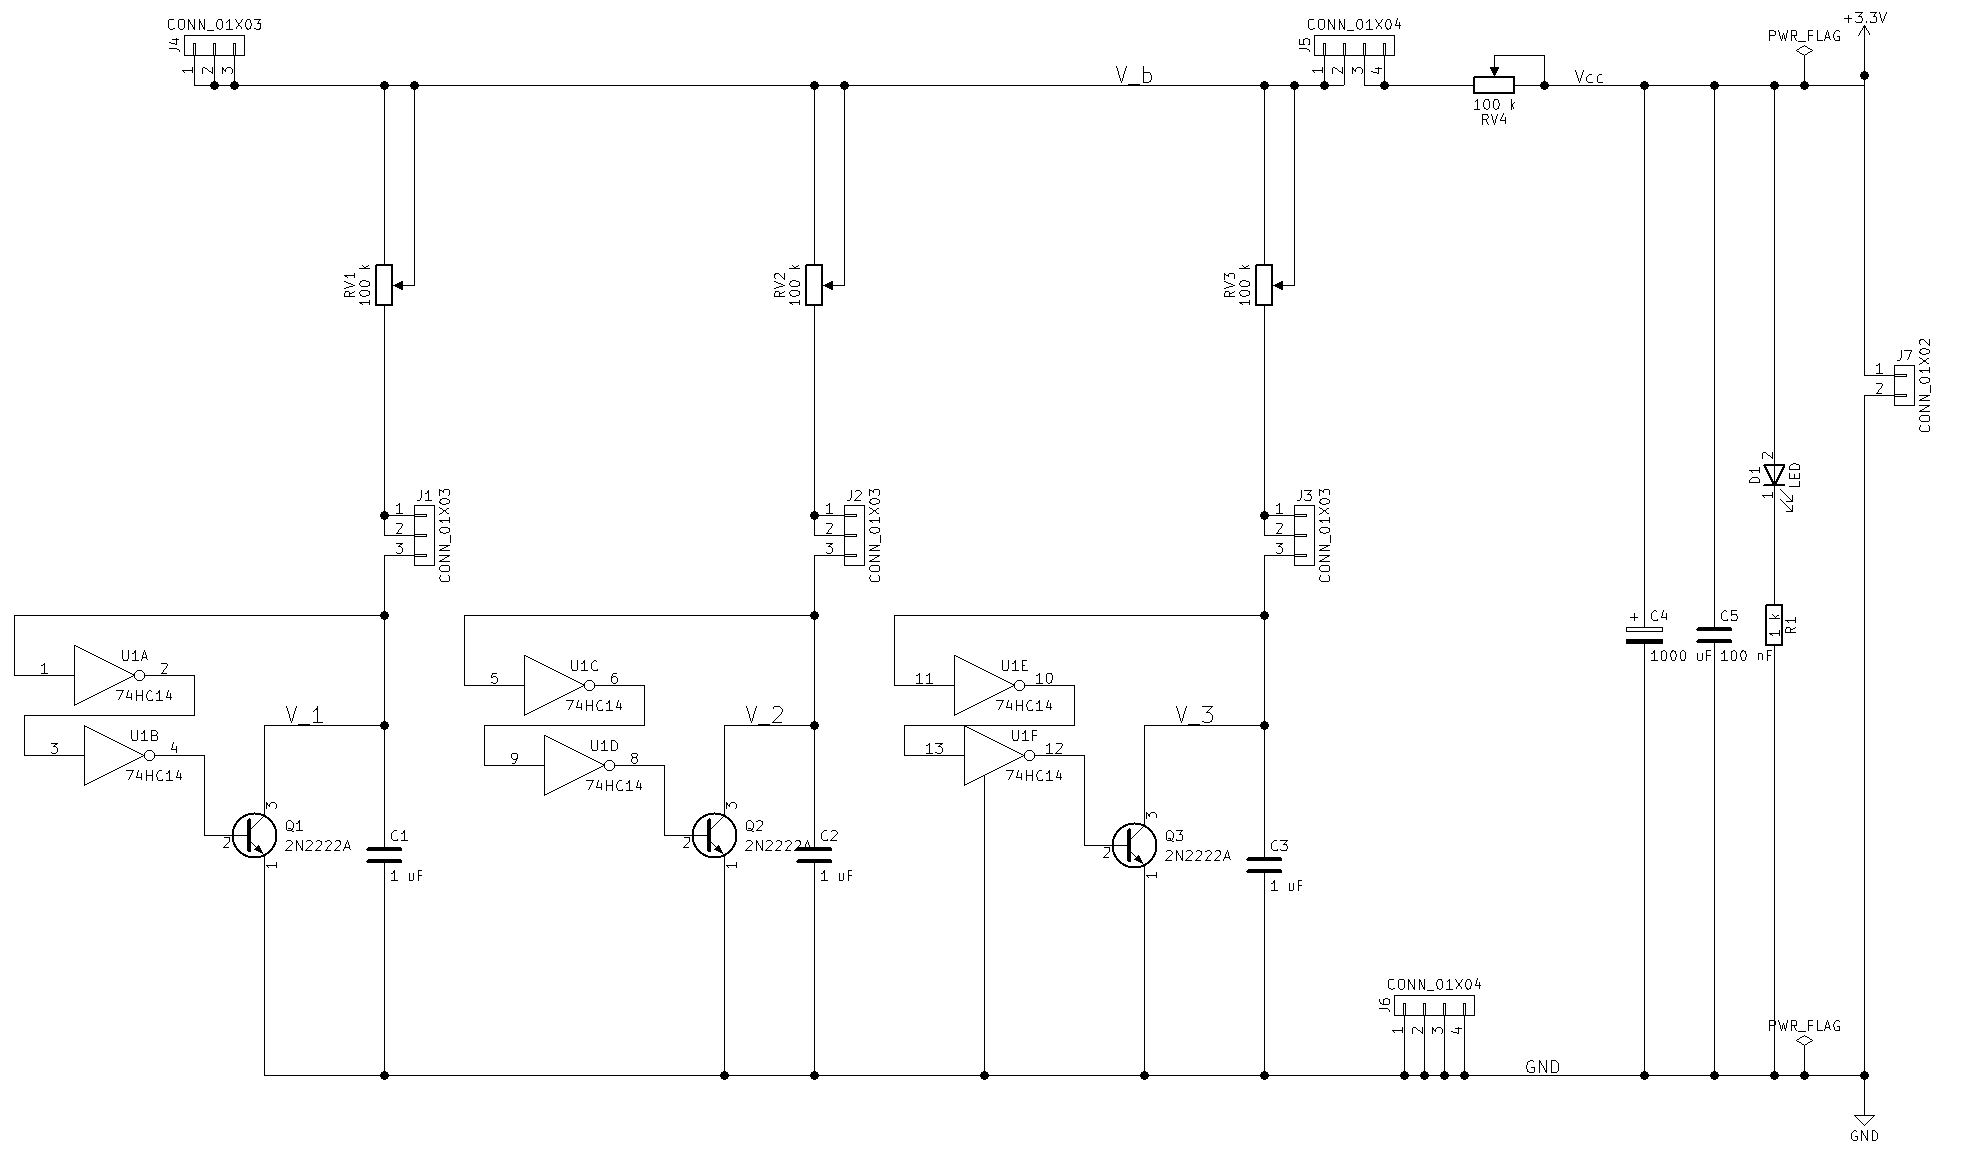
\includegraphics[width=0.9\textwidth]{p/relax3ds_schem.png} }
  \caption{Электрическая схема \RelaxShIi}
  \label{atu:f:relax3ds_schem}
\end{figure}


Динамика.

\section{Модели систем из трёх связанных релаксационных генераторов}

\begin{equation}
  \begin{cases}
    V_b = V_{cc} - R_b ( I_1 + I_2 + I_3 ), \\
      C_1 \dot{V}_1 = \frac{V_b-V_1}{R_{v1}} - \frac{V_1}{R_1} \mathrm{On}_1() - I_{1,\mathrm{leak}}(V_1), \\
      C_2 \dot{V}_2 = \frac{V_b-V_2}{R_{v2}} - \frac{V_2}{R_2} \mathrm{On}_2() - I_{2,\mathrm{leak}}(V_2), \\
      C_3 \dot{V}_3 = \frac{V_b-V_3}{R_{v3}} - \frac{V_3}{R_3} \mathrm{On}_3() - I_{3,\mathrm{leak}}(V_3), \\
      I_i = \frac{V_b-V_i}{R_{vi}}.
  \end{cases}.
    \label{atu:eq:relax3}
\end{equation}

Параметры: \\
$R_b$ --- сопротивление в цепи питания (идентифицируемый параметр), \\
$C_i$ --- ёмкости кождого из релаксационных генераторов, \\
$R_{vi}$ --- сопротивления зарядки релаксационных генераторов, \\
$R_{i}$ --- сопротивления зарядки релаксационных генераторов, \\
$I_{i,\mathrm{leak}}$ --- токи утечки.

Функции $ \mathrm{On}_i() $ определяют моменты переключения генераторов,
задаются алгоритмически (гистерезис). Определяются параметрами
$V_{on}$, $V_{off}$.

\begin{equation}
  \begin{cases}
    V_b = V_{cc} - R_b ( I_1 + I_2 + I_3 ), \\
      C_1 \dot{V}_1 = \frac{V_b-V_1}{R_{v1}} - \frac{V_1}{R_1} \mathrm{On}_1() - \frac{V_1}{R_1+R_{1,\mathrm{leak}}}, \\
      C_2 \dot{V}_2 = \frac{V_b-V_2}{R_{v2}} - \frac{V_2}{R_2} \mathrm{On}_2() - \frac{V_2}{R_2+R_{2,\mathrm{leak}}}, \\
      C_3 \dot{V}_3 = \frac{V_b-V_3}{R_{v3}} - \frac{V_3}{R_3} \mathrm{On}_3() - \frac{V_3}{R_3+R_{3,\mathrm{leak}}}, \\
      I_i = \frac{V_b-V_i}{R_{vi}}.
  \end{cases}.
    \label{atu:eq:relax3_linleak}
\end{equation}

$R_{i,\mathrm{leak}}$ --- сопротивления утечки.



\section{Критерии идентификации систем из трёх связанных релаксационных генераторов}

\begin{figure}[htb!]
  \centerline{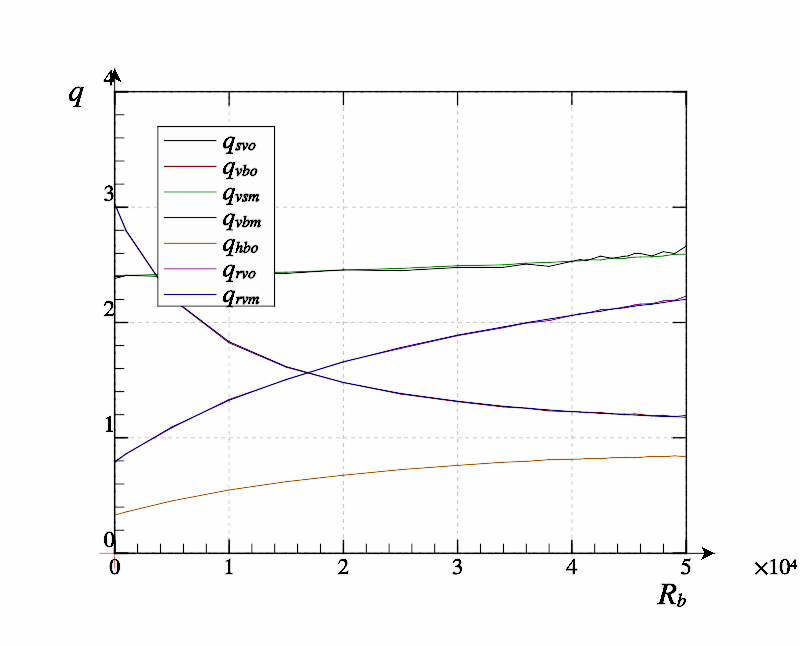
\includegraphics[width=0.7\textwidth]{p/relax3_read_q-p_q1.png} }
  \caption{Зависимости для рассмативаетмых критериев идентификации для системы релаксационных генераторов на паре комплиментарных транзисторов}
  \label{atu:f:relax3d_q}
\end{figure}

\begin{figure}[htb!]
  \centerline{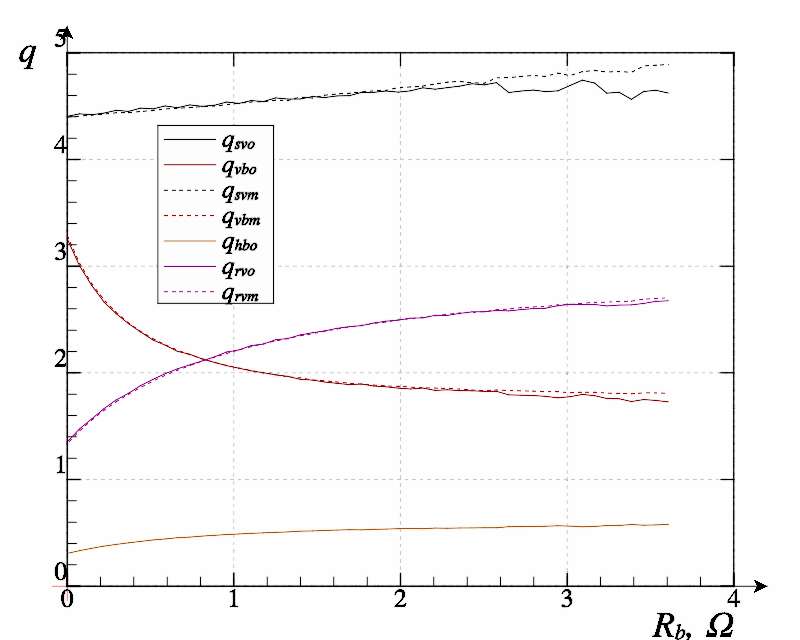
\includegraphics[width=0.7\textwidth]{p/relax3ds_read_q-p_q1.png} }
  \caption{Зависимости для рассмативаетмых критериев идентификации для системы релаксационных генераторов на триггерах Шмидта}
  \label{atu:f:relax3ds_q}
\end{figure}

\section{Идентификация параметра системы из трёх связанных релаксационных генераторов}

\begin{figure}[htb!]
  \centerline{
    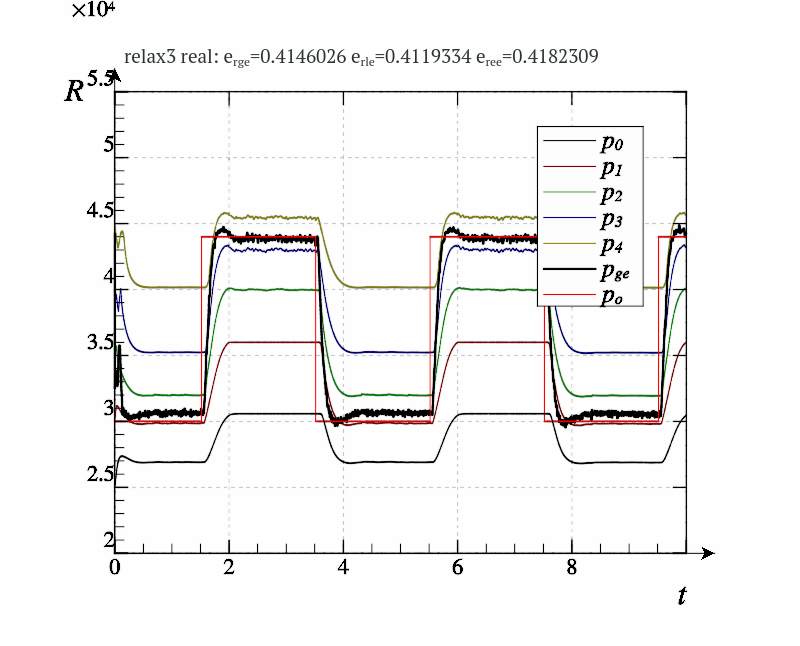
\includegraphics[width=0.45\textwidth]{p/relax3_read_id2-p_p_03.png}
    \hfill
    \includegraphics[width=0.45\textwidth]{p/relax3_read_id2-p_pp_03.png}
  }
  \caption{Идентификация }
  \label{atu:f:relax3d_id}
\end{figure}

\begin{figure}[htb!]
  \centerline{
    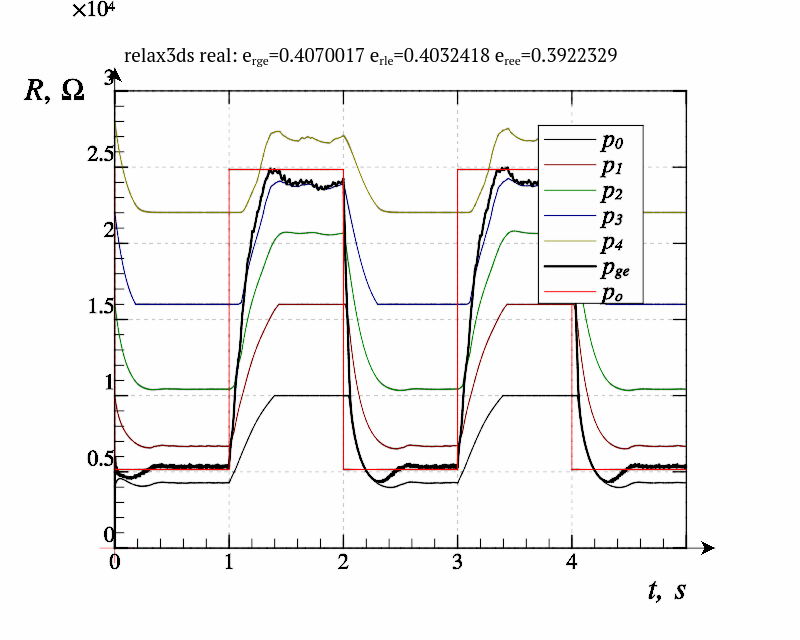
\includegraphics[width=0.45\textwidth]{p/relax3d_read_id2_0-p_p.png}
    \hfill
    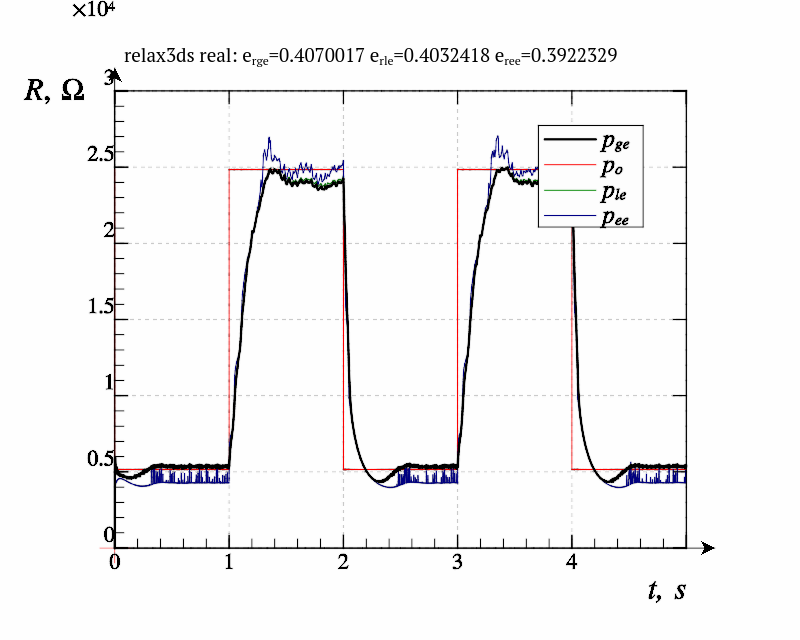
\includegraphics[width=0.45\textwidth]{p/relax3d_read_id2_0-p_pp.png}
  }
  \caption{Идентификация 3ds 0}
  \label{atu:f:relax3ds_id_0}
\end{figure}

\begin{figure}[htb!]
  \centerline{
    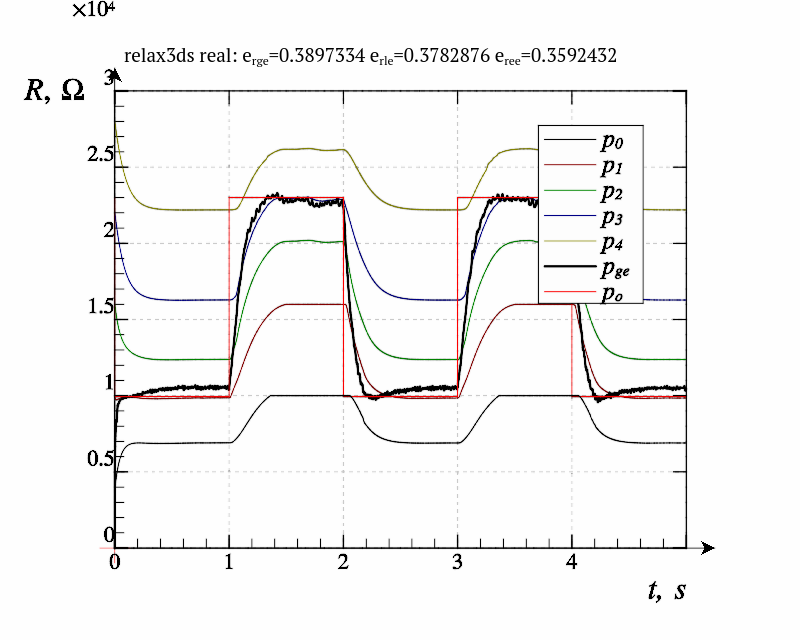
\includegraphics[width=0.45\textwidth]{p/relax3d_read_id2_1-p_p.png}
    \hfill
    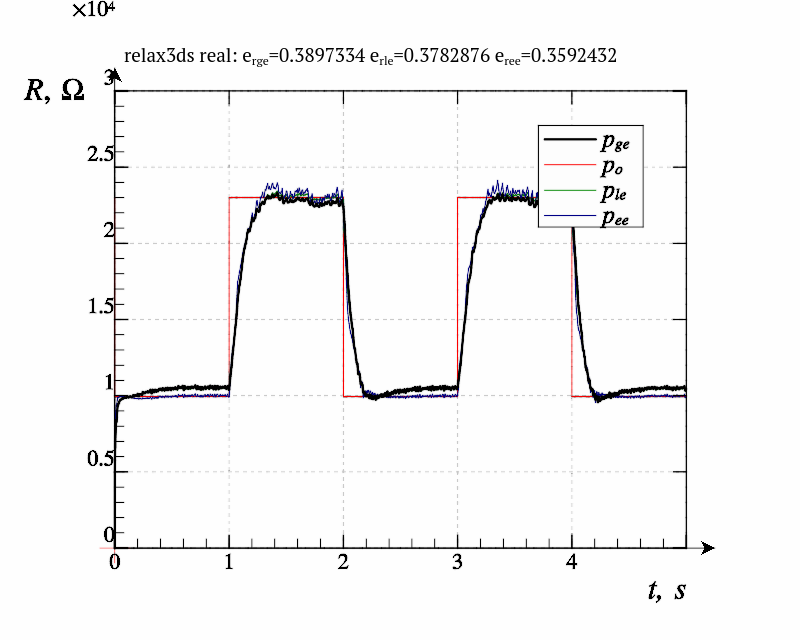
\includegraphics[width=0.45\textwidth]{p/relax3d_read_id2_1-p_pp.png}
  }
  \caption{Идентификация 3ds 1}
  \label{atu:f:relax3ds_id_1}
\end{figure}

\begin{figure}[htb!]
  \centerline{
    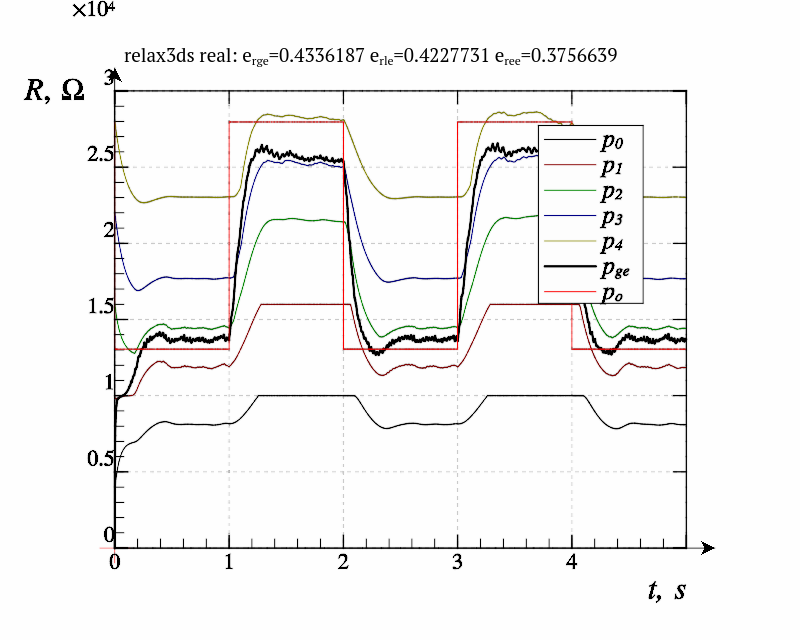
\includegraphics[width=0.45\textwidth]{p/relax3d_read_id2_2-p_p.png}
    \hfill
    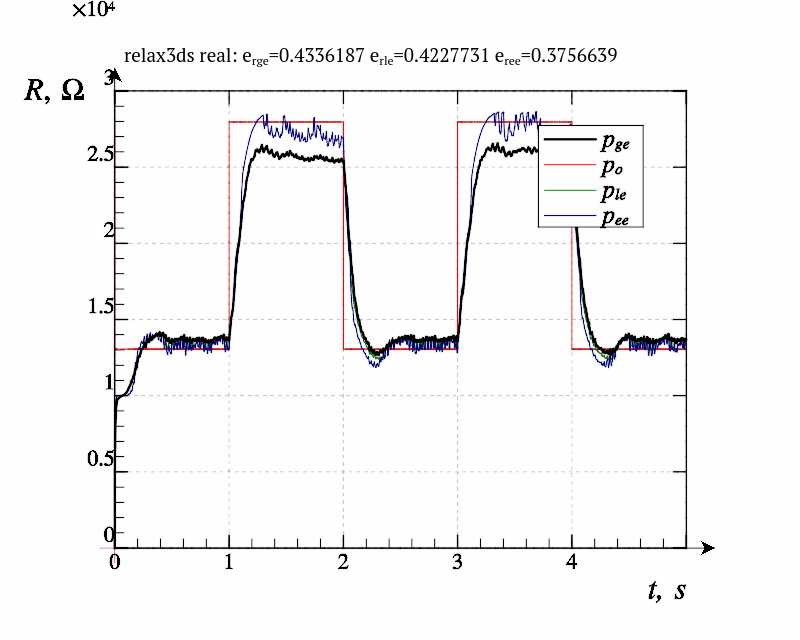
\includegraphics[width=0.45\textwidth]{p/relax3d_read_id2_2-p_pp.png}
  }
  \caption{Идентификация 3ds 2}
  \label{atu:f:relax3ds_id_2}
\end{figure}


\begin{figure}[htb!]
  \centerline{
    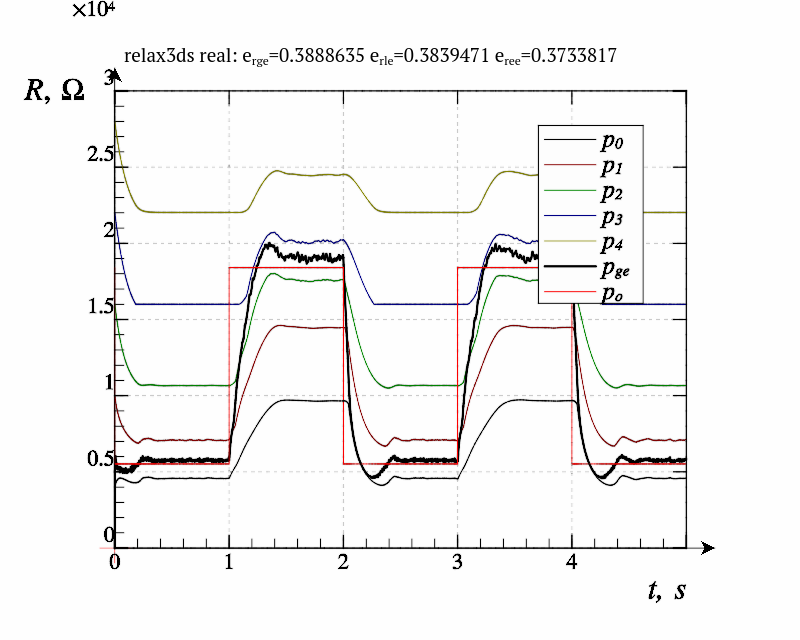
\includegraphics[width=0.45\textwidth]{p/relax3d_read_id2_3-p_p.png}
    \hfill
    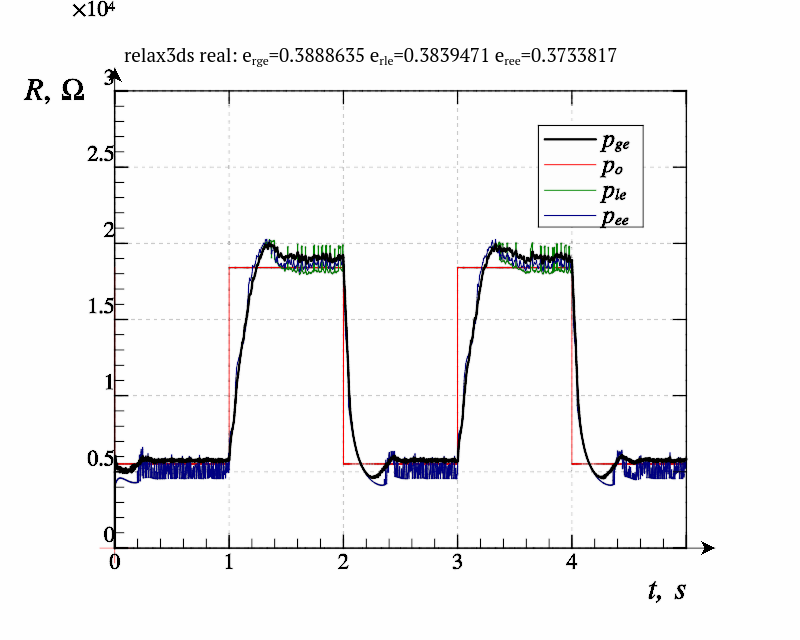
\includegraphics[width=0.45\textwidth]{p/relax3d_read_id2_3-p_pp.png}
  }
  \caption{Идентификация 3ds 3}
  \label{atu:f:relax3ds_id_3}
\end{figure}

\section{Выводы по разделу \thechapter}

Выводы.


